% \documentclass[border=0.2cm]{standalone}

% \usepackage{array}
% \usepackage{stmaryrd}
% \usepackage{amsmath}
% \usepackage{tikz}

% \usetikzlibrary{shapes.geometric, shapes.arrows}

% \begin{document}
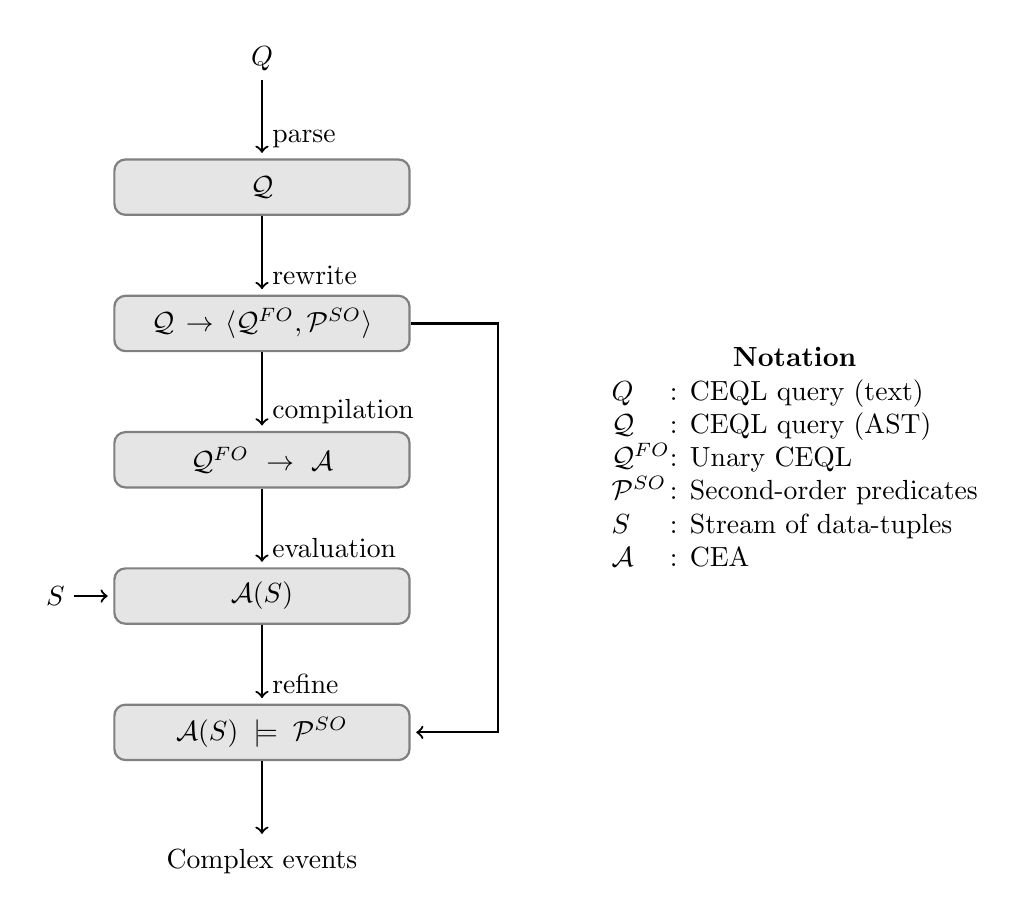
\begin{tikzpicture} [
    auto,
    block/.style    = { rectangle, draw=gray, thick,
                        fill=gray!20, text width=10em, text centered,
                        rounded corners, minimum height=2em },
    line/.style     = { draw, thick, ->, shorten >=2pt },
  ]

  % Nodes as matrix
  \matrix [column sep=5mm, row sep=10mm] {
                    & \node [text centered] (text) {$Q$}; & \\
                    & \node [block] (query) {$\mathcal{Q}$}; & \\
                    & \node [block] (rewrite) {$\mathcal{Q} \to \langle \mathcal{Q}^{FO}, \mathcal{P}^{SO} \rangle $}; \\
                    & \node [block] (compilation) {$\mathcal{Q}^{FO} \to \mathcal{A}$}; & \\
    \node[text centered](stream){$S$}; & \node [block] (evaluation) {${\llbracket \mathcal{A} \rrbracket}(S)$}; & \\
                    & \node [block] (refine) {${\llbracket \mathcal{A} \rrbracket}(S) \models \mathcal{P}^{SO}$}; & \\
                    & \node [text centered] (output) {Complex events}; & \\
  };

  % Edges
  \begin{scope} [every path/.style=line]
    \path (text)         --  node [near end] {parse} (query);
    \path (query)        --  node [near end] {rewrite} (rewrite);
    \path (rewrite)      --  node [near end] {compilation} (compilation);
    \path (compilation)  --  node [near end] {evaluation} (evaluation);
    \path (stream)  --  (evaluation);
    \path (evaluation)  --  node [near end] {refine} (refine);
    \path (rewrite)   --++  (3,0) |- (refine);
    \path (refine)  --  (output);
  \end{scope}

  % Legend
  \node (legend) at (7, 0){
    \begin{tabular}{l@{: }l}
      \multicolumn{2}{c}{\textbf{Notation}} \\
      $Q$ & CEQL query (text) \\
      $\mathcal{Q}$ & CEQL query (AST)\\
      $\mathcal{Q}^{FO}$ & Unary CEQL \\
      $\mathcal{P}^{SO}$ & Second-order predicates \\
      $S$ & Stream of data-tuples \\
      $\mathcal{A}$ & CEA \\
      \end{tabular}
  };
\end{tikzpicture}
% \end{document}
